\documentclass[14pt]{extarticle}
\usepackage[english,ukrainian]{babel}
\usepackage[utf8]{inputenc}
\usepackage{amsmath,amssymb}
\usepackage{parskip}
\usepackage{graphicx}
\usepackage{tcolorbox}
\tcbuselibrary{skins}
\usepackage[framemethod=tikz]{mdframed}
\usepackage{chngcntr}
\usepackage{enumitem}
\usepackage{hyperref}
\usepackage{float}
\usepackage{subfig}
\usepackage{esint}
\usepackage[top=2.5cm, left=3cm, right=3cm, bottom=4.0cm]{geometry}
\usepackage[table]{xcolor}
\usepackage{algorithm}
\usepackage{algpseudocode}
\usepackage{listings}

\title{Індивідуальне завдання з курсу ``Теорія міри''}
\author{Студента 3 курсу групи МП-31 Захарова Дмитра}
\date{\today}

\begin{document}

\maketitle

\section*{Завдання 1}

\textbf{Умова.} Нехай $(\mathbb{R},\mathcal{S}_1,\lambda_1)$ є простором з мірою,
\[
f_n(x) = \begin{cases}
    \arctan x, & x \in [e^{n-\frac{1}{n}},e^n] \\
    0, & x \in \mathbb{R} \setminus [e^{n-\frac{1}{n}},e^n]
\end{cases}, \; x \in \mathbb{R}
\]
З'ясувати:
\begin{enumerate}
    \item Чи є послідовність $\{f_n\}_{n \in \mathbb{N}}$ збіжною м.с. відносно міри $\lambda_1$ на $\mathbb{R}$? Якщо так, то знайти вiдповiдну границю. Вiдповiдь обґрунтувати.
    \item Чи є послідовність $\{f_n\}_{n \in \mathbb{N}}$ збіжною за мірою $\lambda_1$ на $\mathbb{R}$? Якщо так, то знайти вiдповiдну границю. Вiдповiдь обґрунтувати.
\end{enumerate}

\textbf{Розв'язок.} Перед відповідю, зрозуміємо характер послідовності $\{f_n(x)\}_{n \in \mathbb{N}}$. По-перше, область, де задаються ненульові значення, постійно рухається вздовж вісі $Ox$ вправо. Як наслідок, $x$ стає дуже великим і значення функції дуже швидко (насправді буквально з $n=4$) стають близькими до $\lim_{x \to \infty}\arctan x = \frac{\pi}{2}$. 

Проте, цікава властивість таких відрізків це те, що їх довжина не зменьшується і прямує до нескінченності. Дійсно, розглянемо довжину відрізку
\[
L=\lim_{n \to \infty}\left(e^n - e^{n-\frac{1}{n}}\right) = \lim_{x \to 0}\left(e^{\frac{1}{x}} - e^{\frac{1}{x}-x}\right) = \lim_{x \to 0} e^{\frac{1}{x}}\left(1-e^{-x}\right)
\]
Тепер скористаємося тим, що $1-e^{-x} = x - \frac{x^2}{2} + \overline{o}(x^2), x \to 0$:
\[
L = \lim_{x \to 0}xe^{\frac{1}{x}}\underbrace{\left(1 - \frac{x}{2} + x\cdot \overline{o}(1)\right)}_{\alpha(x)} = \lim_{x \to 0} \alpha(x)xe^{\frac{1}{x}}
\]
Отже, маємо добуток функції $\alpha(x)$, що прямує до $1$, а також $xe^{\frac{1}{x}}$. Нескладно показати, що $xe^{\frac{1}{x}}\xrightarrow[x\to 0]{} \infty$, оскільки 
\[
xe^{\frac{1}{x}} = x\left(1 + \frac{1}{x} + \frac{1}{2x^2} + \dots\right) = x + 1 + \underbrace{\frac{1}{2x} + \dots}_{\to \infty \, \text{для} \, x \to 0}
\]
Тому добуток теж прямує до $\infty$. Отже, $L=+\infty$. 

Сам графік $f_n$ для $n=1,\dots,5$ зображено на рис. \ref{fig:plot}.

\begin{figure}[H]
    \centering
    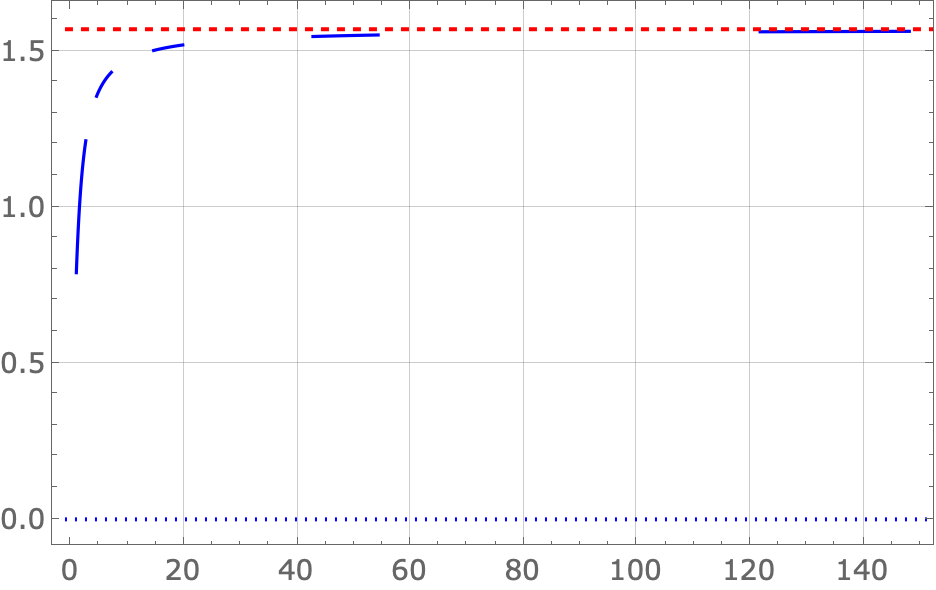
\includegraphics[width=0.7\textwidth]{images/final_2.png}
    \caption{Перші 5 функцій $f_n$}
    \label{fig:plot}
\end{figure}

\textbf{Пункт 1.} Помітимо, що
\[
\forall x \in \mathbb{R} \; \exists n_x \in \mathbb{N} \; \forall n \geq n_x: f_n(x) = 0
\]
Дійсно, достатньо
\[
n_x := \min\left\{n \in \mathbb{N}: e^{n-\frac{1}{n}} > x\right\}
\]
В такому разі, $\forall x \in \mathbb{R}:\lim_{n \to \infty}f_n(x) = 0$, що автоматично означає збіжність до $0$ майже скрізь (тобто $f_n = 0 \, (\text{mod} \, \lambda_1)$). 

\textbf{Пункт 2.} За означенням, збіжність послідовності $\{f_n\}_{n \in \mathbb{N}}$ означає:
\[
\exists f: f_n \xrightarrow[]{\lambda_1} f \iff \forall \varepsilon > 0: \lambda_1\left(\{x \in \mathbb{R}: |f_n(x)-f(x)| \geq \varepsilon\}\right) \xrightarrow[n \to \infty]{} 0
\]
Візьмемо $f\equiv 0$, тоді
\[
\forall \varepsilon > 0: \lim_{n \to \infty} \lambda_1(\{x \in \mathbb{R}: |f_n(x)| \geq \varepsilon\}) = 0
\]
Візьмемо достатньо малий $\varepsilon$, наприклад, для конкретики, $\varepsilon=\frac{1}{10}$. Тоді
\[
U_{\varepsilon}^{(n)}:=\{x \in \mathbb{R}: |f_n(x)| \geq 0.1\} = [e^{n-\frac{1}{n}},e^n]
\]
Проте, оскільки $e^n-e^{n-\frac{1}{n}}\xrightarrow[n \to \infty]{}+\infty$, то і $\lim_{n \to \infty}\lambda_1(U_{\varepsilon}^{(n)}) = +\infty$. Отже, $f$ не є збіжною на $\mathbb{R}$.

\textbf{Відповідь.} $f$ не є збіжною, але є майже скрізь збіжною до $0$.

\pagebreak

\section*{Завдання 2}
\textbf{Умова.} Обчислити інтеграл
\[
\int_{\mathbb{R}^+} \frac{d\lambda_1(x)}{[3x+1][3x+4]}
\]
\textbf{Розв'язок.} Помітимо, що
\[
\mathbb{R}^+ = \bigcup_{n \in \mathbb{N}} A_n, \; A_n = \left[\frac{n-1}{3},\frac{n}{3}\right)
\]
Оскільки $\{A_n\}_{n \in \mathbb{N}}$ є попарно неперетинними, то можемо застосувати $\sigma$-адитивність інтеграла Лебега і отримати
\[
\mathcal{I} := \int_{\mathbb{R}^+}\frac{d\lambda_1(x)}{[3x+1][3x+4]} = \sum_{n \in \mathbb{N}}\int_{A_n} \frac{d\lambda_1(x)}{[3x+1][3x+4]}
\]
Тепер помітимо, що для усіх $x$ з $A_n$, значення $n \leq 3x+1 < n+1$, тому $[3x+1]=n$. Аналогічним чином $[3x+4]=n+3$. Отже
\[
\mathcal{I} = \sum_{n \in \mathbb{N}} \int_{[\frac{n-1}{3},\frac{n}{3})} \frac{d\lambda_1(x)}{n(n+3)} = \sum_{n \in \mathbb{N}} \frac{1}{n(n+3)}\int_{[\frac{n-1}{3},\frac{n}{3})}d\lambda_1(x)
\]
Далі користуємось властивістю інтеграла Лебега $\int_{[\alpha,\beta)}d\lambda_1(x)=\beta-\alpha$, тому
\[
\mathcal{I} = \frac{1}{3}\sum_{n \in \mathbb{N}}\frac{1}{n(n+3)} = \frac{1}{3}\sum_{n \in \mathbb{N}}\left(\frac{1}{3n}-\frac{1}{3(n+3)}\right) = \frac{1}{9}\sum_{n \in \mathbb{N}}\left(\frac{1}{n}-\frac{1}{n+3}\right)
\]
Якщо позначимо $S_m := \sum_{n=1}^{m}\left(\frac{1}{n}-\frac{1}{n+3}\right)$, то $\mathcal{I} = \frac{1}{9}\cdot\lim_{m \to \infty}S_m$. Отже, для достатньо великих $m$:
\begin{gather*}
S_m = \sum_{n=1}^m \left(\frac{1}{n}-\frac{1}{n+3}\right) = \sum_{n=1}^m \frac{1}{n} - \sum_{n=1}^m \frac{1}{n+3}\\
= \sum_{n=1}^m \frac{1}{n} - \sum_{n=4}^{m+3} \frac{1}{n} = 1 + \frac{1}{2} + \frac{1}{3} - \underbrace{\frac{1}{m+1}-\frac{1}{m+2}-\frac{1}{m+3}}_{\to 0} \xrightarrow[m \to \infty]{} \frac{11}{6}
\end{gather*}
\textbf{Відповідь.} $\frac{11}{54}$.

\section*{Завдання 3}

\textbf{Умова.} Обчислити границю
\[
\lim_{n \to \infty} \int_{\mathbb{R}^+} \frac{n\left(e^{-\frac{x^3}{n}}-1\right)}{(1+x^4)^2}d\lambda_1(x)
\]

\textbf{Розв'язок.} Позначимо
\[
\mathcal{J}_n := \int_{\mathbb{R}^+} \frac{n\left(e^{-\frac{x^3}{n}}-1\right)}{(1+x^4)^2}d\lambda_1(x)
\]
\textbf{Спосіб 1.} Помітимо, що
\[
\forall x \in \mathbb{R}^+: 1 - \frac{x^3}{n} \leq e^{-\frac{x^3}{n}} \leq 1-\frac{x^3}{n} + \frac{x^6}{2n^2},
\]
тому, застосовуючи теорему про порівняння інтегралів Лебега, отримуємо
\[
-\int_{\mathbb{R}^+}\frac{x^3 d\lambda_1(x)}{(1+x^4)^2} \leq \mathcal{J}_n \leq \int_{\mathbb{R}^+} \frac{-x^3 + \frac{x^6}{2n}}{(1+x^4)^2}d\lambda_1(x)
\]
Інтеграл ліворуч є інтегрованим по Ріману, а отже, за теоремою про порівняння інтеграла Рімана та Лебега, по Лебегу також. Робимо заміну $z=1+x^4$, тоді $dz=4x^3dx$, тому
\[
-\int_{\mathbb{R}^+} \frac{x^3dx}{(1+x^4)^2} = -\frac{1}{4}\int_{[1,+\infty)} \frac{dz}{z^2} = \frac{1}{4}\left(\frac{1}{z}\right)\Big|_{z=1}^{z\to+\infty} = -\frac{1}{4}
\]
Тепер знайдемо інтеграл праворуч:
\[
\int_{\mathbb{R}^+} \frac{-x^3+\frac{x^6}{2n}}{(1+x^4)^2}d\lambda_1(x) = \underbrace{-\int_{\mathbb{R}^+} \frac{x^3d\lambda_1(x)}{(1+x^4)^2}}_{=-\frac{1}{4}} + \frac{1}{2n}\int_{\mathbb{R}^+} \frac{x^6d\lambda_1(x)}{(1+x^4)^2}
\]
Помітимо, що вираз $\int_{\mathbb{R}^+}\frac{x^6d\lambda_1(x)}{(1+x^4)^2} < +\infty$, оскільки підінтегральний вираз пропорційний $\frac{1}{x^2}$. Причому, значення цього інтеграла не залежить від $n$, тому позначимо $\gamma := \int_{\mathbb{R}^+}\frac{x^6d\lambda_1(x)}{(1+x^4)^2}$ (справжнє значення, згідно \textit{Wolfram Mathematica}, $\gamma=\frac{3\pi}{8\sqrt{2}}$, але точно знати нам його не обов'язково). Тому отримаємо:
\[
-\frac{1}{4} \leq \mathcal{J}_n \leq -\frac{1}{4} + \frac{\gamma}{2n} \implies \boxed{\lim_{n \to \infty}\mathcal{J}_n = -\frac{1}{4}}
\]

\textbf{Спосіб 2.} Помітимо, що
\[
n\left(e^{-\frac{x^3}{n}}-1\right) \to -x^3 \; (\text{mod} \, \lambda_1).
\]
Тоді за теоремою Лебега про мажоровану збіжність,
\[
\lim_{n \to \infty}\int_{\mathbb{R}^+} \frac{n\left(e^{-\frac{x^3}{n}}-1\right)}{(1+x^4)^2}d\lambda_1(x) = \int_{\mathbb{R}^+} \frac{-x^3 d\lambda_1(x)}{(1+x^4)^2} = -\frac{1}{4}
\]
\textbf{Доведення збіжності м.с.} Для цього розглянемо границю
\[
\lim_{n \to \infty} n\left(e^{-\frac{x^3}{n}}-1\right) = \lim_{\epsilon \to 0} \frac{e^{-\epsilon x^3} - 1}{\epsilon} = \lim_{\epsilon \to 0} \frac{-\epsilon x^3 + \overline{o}(\epsilon x^3)}{\epsilon} = x^3\lim_{\epsilon \to 0}(-1 + \overline{o}(1)) = -x^3
\]
Отже для усіх $x \in \mathbb{R}^+$ маємо $\lim_{n \to \infty} n\left(e^{-\frac{x^3}{n}}-1\right)=-x^3$.

\textbf{Відповідь.} $-\frac{1}{4}$.

\end{document}

